\chapter{Introduction}
Since the advent of Web 2.0, users have increasingly created content, but also contributed reactions to content in the form of comments. Comments are challenging to analyze due to their short lengths and informal style, meaning that any individual comment provides very little data to work with and is highly variable. However, comments capture innate and an explicit opinion of a user that makes it invaluable towards personalization. In this work, we explore the possibilities of exploiting comments towards the end of personalized recommendations.

\section{The Recommendation Paradox}
Conventional recommender systems make use of explicit user ratings on items and where ratings are not available, they make use of clicks. For further personalization, clicks are often enriched with metadata regarding the item, for instance tags. In addition, many web applications do not make use of an explicit `dislike' button as this is often conceived as offending the original author of the item. While there exists a `like' button which in most cases implicates a good recommendation was received, there is no direct way to capture the opposite.

Consider the case of a cold state scenario where a new user probes the system and clicks on one of the top recommendations and the user did not like want was presented in the item either because the original title to the item was misleading or he had accidentally clicked on it. In a naive click based recommendation, the user is immediately flooded with similar items. As most web applications often tie the hands of users by not providing explicit `dislike' feedback, they then turn to the only possible way of expressing their discontent - comments.

\ldots

\section{Overview of State-Of-Art}
\subsection{Collaborative Filtering}
\subsection{Content Based Filtering}
\subsection{Hybrid Filtering}

\newpage
\section{Research Flow}
\begin{figure}[!h]
\centering
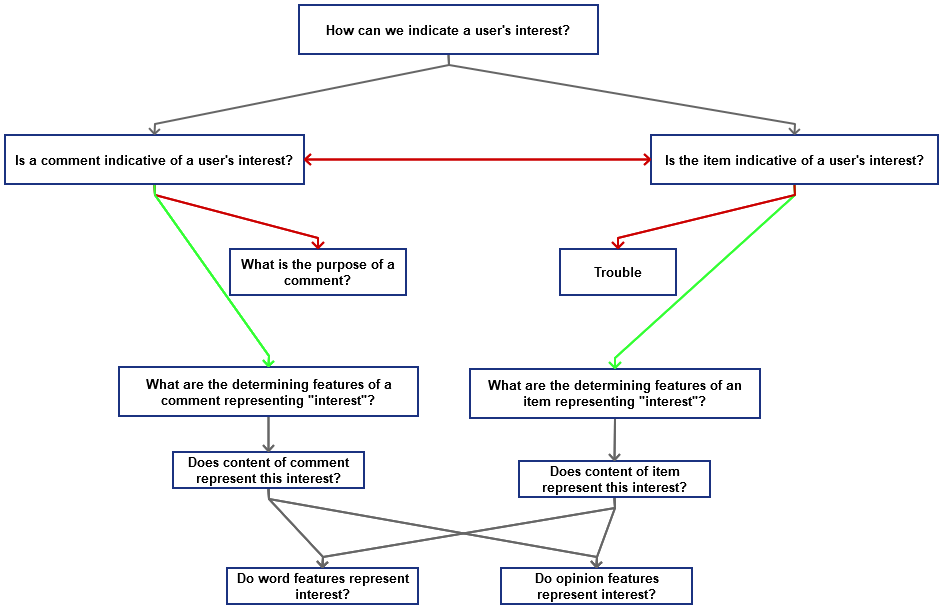
\includegraphics[width=1\textwidth]{c-1_images/r_questions_rep.png}
\caption{Representation of Interest}
\label{fig:r_questions_rep}
\end{figure}

\begin{figure}[!h]
\centering
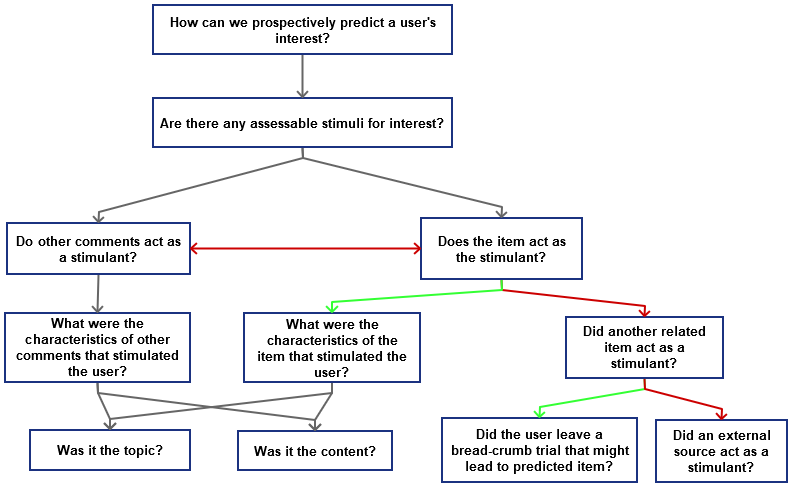
\includegraphics[width=0.8\textwidth]{c-1_images/r_questions_pred.png}
\caption{Prediction of Interest}
\label{fig:r_questions_pred}
\end{figure}

\begin{figure}[!h]
\centering
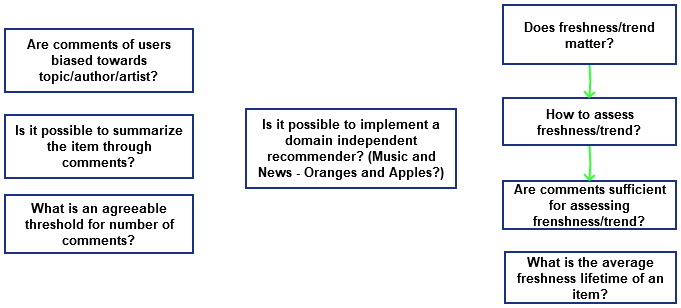
\includegraphics[width=0.7\textwidth]{c-1_images/r_questions_misc.png}
\caption{Miscellaneous}
\label{fig:r_questions_misc}
\end{figure}